\documentclass[12pt,oneside]{book}
\usepackage[letterpaper, left=1.2in, right=1.2in, top=1cm, bottom=1in]{geometry}
\pagestyle{plain}
\usepackage[pagestyles]{titlesec}
\usepackage{titletoc}
\usepackage{tocloft}
\usepackage{graphicx}
\usepackage{caption}
\setcounter{secnumdepth}{4}
\usepackage[backend=biber,style=apa,sorting=nyt]{biblatex} % apa citation style
\addbibresource{Reference.bib}
\usepackage[utf8]{inputenc}
\usepackage{appendix}
\usepackage{listings}
\usepackage{bm}
\titleformat{\chapter}%
  {\normalfont\bfseries\Huge}{\thechapter.}{10pt}{}
\newpagestyle{mystyle}{
  \sethead[][\thechapter.\enspace\chaptertitle][]{}{\thesection~\sectiontitle}{}
\setfoot{}{\thepage}{}}
\AtBeginDocument{\renewcommand{\bibname}{References}}

\captionsetup[figure]{margin=1.5cm,font=small,labelfont={bf},name={Figure},labelsep=colon,textfont={it}}
\captionsetup[table]{margin=1.5cm,font=small,labelfont={bf},name={Table},labelsep=colon,textfont={it}}

\begin{document}

%%%%%%%%%%%%%%%%%%%%%%%%%%%%%%%%%%%%%%%%%%
%% Additional Material
%%%%%%%%%%%%%%%%%%%%%%%%%%%%%%%%%%%%%%%%%%

%========================================
% Title Page
%========================================
%% Define your thesis title, your name, your department, your degree, and your month and year of graduation here

\newcommand{\Contributers}{James Thomas - 9195071 \\ Liam Smith - SID \\ Alexander Collins - SID}
\newcommand{\Module}{360CT - Advanced Network Management and Design}



%%%%%%%%%%%%%%%%%%%%%%%%%%%%%%%%%%%%%%%%%%%%%%%%%%%%%%%%%
% Do not edit these lines unless you wish to customize the template
%%%%%%%%%%%%%%%%%%%%%%%%%%%%%%%%%%%%%%%%%%%%%%%%%%%%%%%%%

\begin{titlepage}
\begin{center}

\begin{center}
    
\includegraphics[width=0.3\columnwidth, keepaspectratio]{Additional/cov_logo.png}\\
\end{center}

\hspace{0pt}
\vfill
\begin{huge}
Yotsuba Network Design Brief\\
\vspace{\baselineskip}
\Module\\
\end{huge}
\vspace{\baselineskip}
By\\
\Contributers\\
\vspace{\baselineskip}
\vfill
\hspace{0pt}

\end{center}
\end{titlepage}
\pagenumbering{roman}
\setcounter{page}{2}

%========================================
% Table of Contents
%========================================
\pagenumbering{roman} % Uncomment if Copyright and Acknowledgements are not in use
\setcounter{page}{2} % Uncomment if Copyright and Acknowledgements are not in use
\addcontentsline{toc}{chapter}{Table of Contents}
% \begin{doublespacing}
\tableofcontents
\clearpage
% \end{doublespacing}
% \currentpdfbookmark{Table of Contents}{TOC}

%%%%%%%%%%%%%%%%%%%%%%%%%%%%%%%%%%%%%%%%%%
%% Main Content
%%%%%%%%%%%%%%%%%%%%%%%%%%%%%%%%%%%%%%%%%%

% resume page numbering for rest of document
\pagenumbering{arabic}
\setcounter{page}{1} % set the page number appropriately

\chapter{Introduction}
The purpose of this report is to provide Yotsuba Group with a network design for their new headquarters. Throughout this report, issues arising from the relocation of the headquarters, as well as problems with the network design are identified and addressed in the sections below:
\begin{itemize}
    \item Identifying the requirements of the new network
    \item The devices that will be used to implement the new network
    \item Proposal of a logical network design, including floorplans
    \item An addressing scheme for the network design
    \item Discussion of appropriate policies following relocation
    \item Discussion of network security threats
    \item A plan for network and performance monitoring
    \item Identifying risks and a disaster management plan.
\end{itemize}
We have also taken into consideration the possibility of renting one of the floors to an external company, as well as being able to connect to the old headquarters to cope with expansion.
\chapter{Requirements and Assumptions}

\section{Expansion}
Yotsuba Group is a company experiencing rapid growth, hence the need for their new office space. It is assumed that this rapid expansion is to be around 10-20 new employees per year. Because of this, there is a strong requirement for scalability, so the network can cope with this growth and there are no detrimental effects on network performance. It should be kept in mind that the selection of devices and routing protocols should support this need for scalability.
\section{Network Speeds and Bandwidth}
Research showed that private internet for the greater Tokyo region had available speeds in the range of 10Mbps to 1Gbps. It is assumed that enterprise internet speeds will be within a similar range and that the Yotsuba Group will be purchasing at the top range. Therefor a 10Gbps connection will be used for the designs.
\section{Employee breakdown}
As no information on individual department employee count was provided it has been assumed based on departmental needs.
\begin{itemize}
    \item Research and Technology - 50 employees
    \item Financial Planning - 20 employees
    \item Sales - 34 employees
    \item Material and Design - 50 employees
    \item Personnel - 10 employees
    \item Planning and Manufacturing - 60 employees
    \item Legal and Accounting - 10 employees
    \item Marketing - 20 employees
    \item IT - 16 employees
    \item Department Head and Assistants - 16 (8+8) employees
\end{itemize}
\section{Cisco in Japan}
The network will be using Cisco hardware, some of which will be transferred from the old 
building. A Cisco press release demonstrates how the company plans to transition further into Japan through an agreement between the Japanese Government and Cisco on mass-scale digitalisation projects \parencite{cisco-japan}.
\section{Physical Office Dimensions}
For floors U1, U2, G, 1, 2, 3, 4, 5, 6: 30mx50m , 7m2 per workstation area.
Floor 7: 50mx20m for offices, 25x10m for the meeting room. \\
Floor 7 Balcony: 25mx10m \\
The space provided to each employee workstation area was calculated via an online tool \parencite{floor-space}.
\section{Underground Carpark}
We are assuming that the two-floor underground car park does not currently have a good mobile signal for 3/4g internet access and therefore, Wi-Fi APs should be implemented underground. This  would be helpful for employees who have parked underground as they can still make calls, send emails or do other work from their cars.
\section{Previous Devices}
Some devices such as layer 2 switches and workstations have been transferred from the old office to the new site. This is covered in more detail in section 3. 
\section{Previous Security Threats}
The Yotsuba Group reported a number of security incidents in the last 6 months. These have been assumed below.
\subsection{IP Theft}
The company had some intellectual property stolen from a physical attack on the servers within the company premises, the attackers were not found or apprehended as the security was not to standard. This attack was made possible by a lack of physical security measures on there network infrastructure.
\subsection{Internal Breach}
30\% of attacks come from employee's within the companies, some data was accessed by departments who has access to other parts of the organisation that they should not have had. A lack of access control was the cause of this attack.

\chapter{Physical Network Design}

\section{Devices}
\subsection{Workstations}
It is assumed that all workstations in use have been bought over from the old branch to reduce on cost. The only upgrade that would have to be made to each workstation is the installation of an SFP+ network adaptor. The recommended PCI expansion card is the \emph{ASUS 10GbE SFP+ PCIe 3.0 Network Adapter}. This recommendation is due to high reviews and a reputable manufacturer.
\subsection{Servers}
Any servers needed in the network such as email, DNS or vpn will be generic Linux based draws stored in the server room. Inside the network these servers will be placed within the DMZ area.
\subsection{Wireless Access Points (WAP)}
The Cisco Catalyst 9136 WAP has been chosen for its ability to use WiFi 6, further future-proofing our network solution.
\subsection{Media Converter}
When applicable for use the TP-Link MC220L media converter will be used to allow for use of copper cabling. An example of this use case would be the connection from switch to WAP as the WAP does not have an SFP+ port.
\subsection{Layer 3 Switch}
\subsubsection{Chassis - C4506-E}
It has been assumed that this is a switch that has been bought over from the old building to save on costs. It is an older model that is no longer sold but is going to be supported by Cisco until 2025 \parencite{cisco-4506}.
\subsubsection{Line Card - WS-X4712-SFP+E5}
This line card has been chosen because it can handle the speed of the network while being able to fit multiple in the chosen layer 3 chassis.
\begin{table}[H]
    \centering
    \begin{tabular}{|cccc|}
    \hline
    \multicolumn{1}{|c|}{SKU} & \multicolumn{1}{c|}{Ports} & \multicolumn{1}{c|}{Speed} & Connector \\ \hline
    WS-X4712-SFP+E5           & 12                         & 10GBASE-R                  & SFP+/SFP  \\ \hline
    \end{tabular}
\end{table}
\subsection{Layer 2 Switch}
\subsubsection{Chassis - C9404R}
This chassis has been chosen as it is the correct size needed to fit two supervisor cards and two line cards. This allows for the correct number of ports as well as additional for company expansion. Going any larger would not be beneficial and cost more. 
\subsubsection{Line Card - C9400-LC-48XS}
This line card has been chosen for the access layer switch as we can fit two of them in the chosen chassis. This will provide enough ports to cover the existing devices on each floor as well as any new devices bought in due to expansion.
\begin{table}[H]
    \begin{tabular}{|ccccc|}
    \hline
    \multicolumn{1}{|c|}{SKU} & \multicolumn{1}{c|}{Ports} & \multicolumn{1}{c|}{Connector} & \multicolumn{1}{c|}{Speed} & Total Needed \\ \hline
    C9400-LC-48XS             & 48                         & SFP/SFP+                       & 1/10Gbps                   & 2            \\ \hline
    \end{tabular}
\end{table}
\subsubsection{Supervisor Card - C9400-SUP-1XL-Y}
Allows for 10Gbps on each port.
\subsection{Router}
Cisco 4000 Series Integrated Services Router
\subsection{Firewall}
Cisco Firepower 4125
\section{Wiring}
A full fiber solution will be employed for this network to account for future proofing and to reduce noise on the network.
\subsection{Multimode Fiber - OM4}
The current network will be 10GBASE-SR, using OM4 fiber cables. Using OM4 fiber will give us options to expand to 40GBASE-SR or 100GBASE-SR in future also.
As the solution planned for this building is mostly copperless, OM4 cables will run between all three layers of our network model.
While the distance of 550m at 10Gbps for OM4 is overkill for a 7 story building, the allowance for higher distances at higher speeds (100m at 100Gbps) will be good for future-proofing our solution.
The cost of fiber has been decreasing steadily over the past years, due to this there will not be much of a difference between the cost of copper and fiber ethernet solutions. The only additional cost over a copper solution will be the installation of fiber network adaptors in workstation PCs.
\begin{table}[H]
    \centering
    \begin{tabular}{|ccccc|}
    \hline
    \multicolumn{1}{|c|}{\multirow{2}{*}{Designation}} & \multicolumn{4}{c|}{Distance (m)}                                                                                \\ \cline{2-5} 
    \multicolumn{1}{|c|}{}                             & \multicolumn{1}{c|}{1000BASE-SR} & \multicolumn{1}{c|}{10GBASE-SR} & \multicolumn{1}{c|}{40GBASE-SR} & 100GBASE-SR \\ \hline
    OM1                                                & 300                            & 33                              & N/A                             & N/A         \\ \hline
    OM2                                                & 600                            & 82                              & N/A                             & N/A         \\ \hline
    OM3                                                & 1000                           & 300                             & 100                             & 100         \\ \hline
    OM4                                                & 1100                           & 550                             & 150                             & 150         \\ \hline
    OM5                                                & 1100                           & 550                             & 150                             & 150         \\ \hline
    \end{tabular}
    \caption{Table of distances for Multimode Fiber cables.}
    \label{tab:fiber_distance}
\end{table}
\subsection{Uninterruptible Power Supply}

\section{Device Placement}
\subsection{Patch Pannels}
Patch pannels will be placed on each floor to house access section L2 switches. This allows for the creation of several points of failure, as opposed to a single point of failure of storing all switches in the server room.
\subsection{Ground Floor}
\begin{figure}[H]
    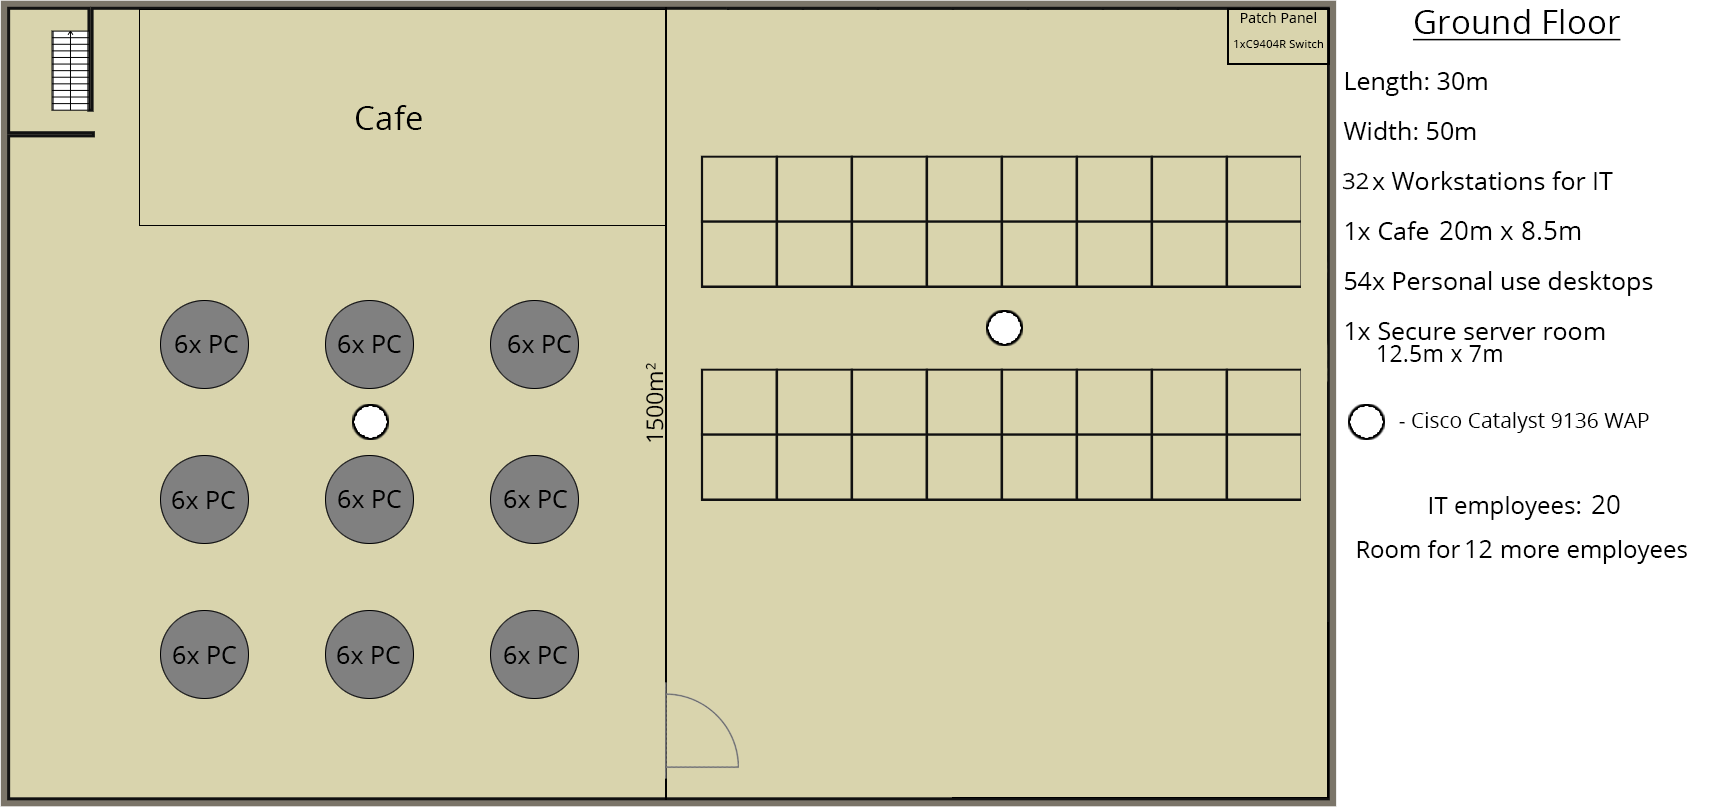
\includegraphics[width=15cm]{Figures/ground.png}
    \caption{Ground floor plan}
    \label{fig:ground_floor}
\end{figure}
\subsection{1st Floor}
\begin{figure}[H]
    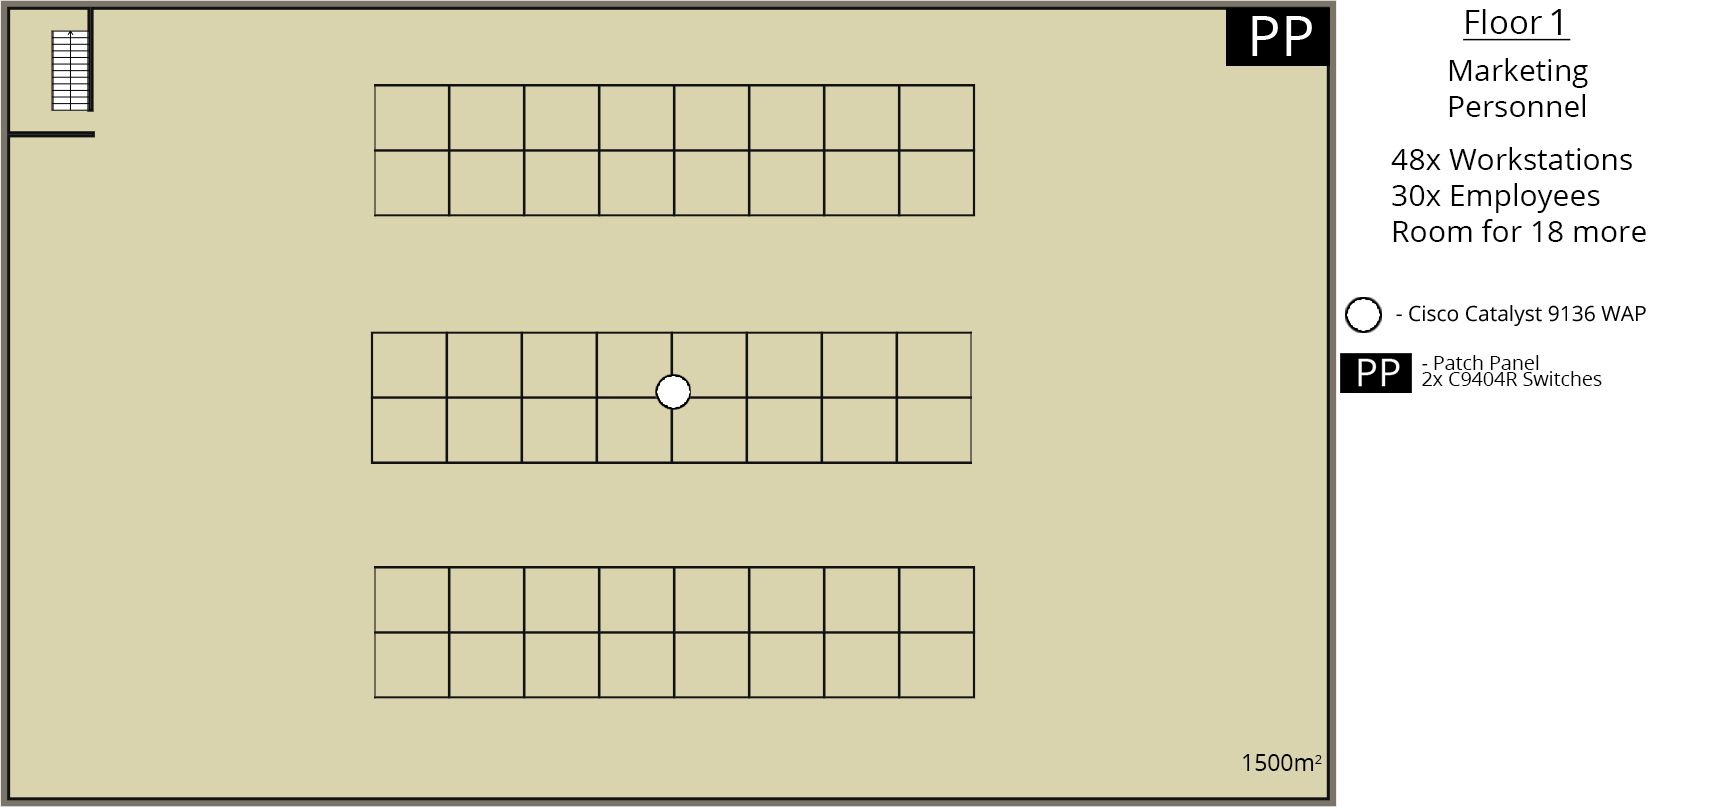
\includegraphics[width=15cm]{Figures/1st-floor.png}
    \caption{1st floor plan}
    \label{fig:1st_floor}
\end{figure}
\subsection{2nd Floor}
\begin{figure}[H]
    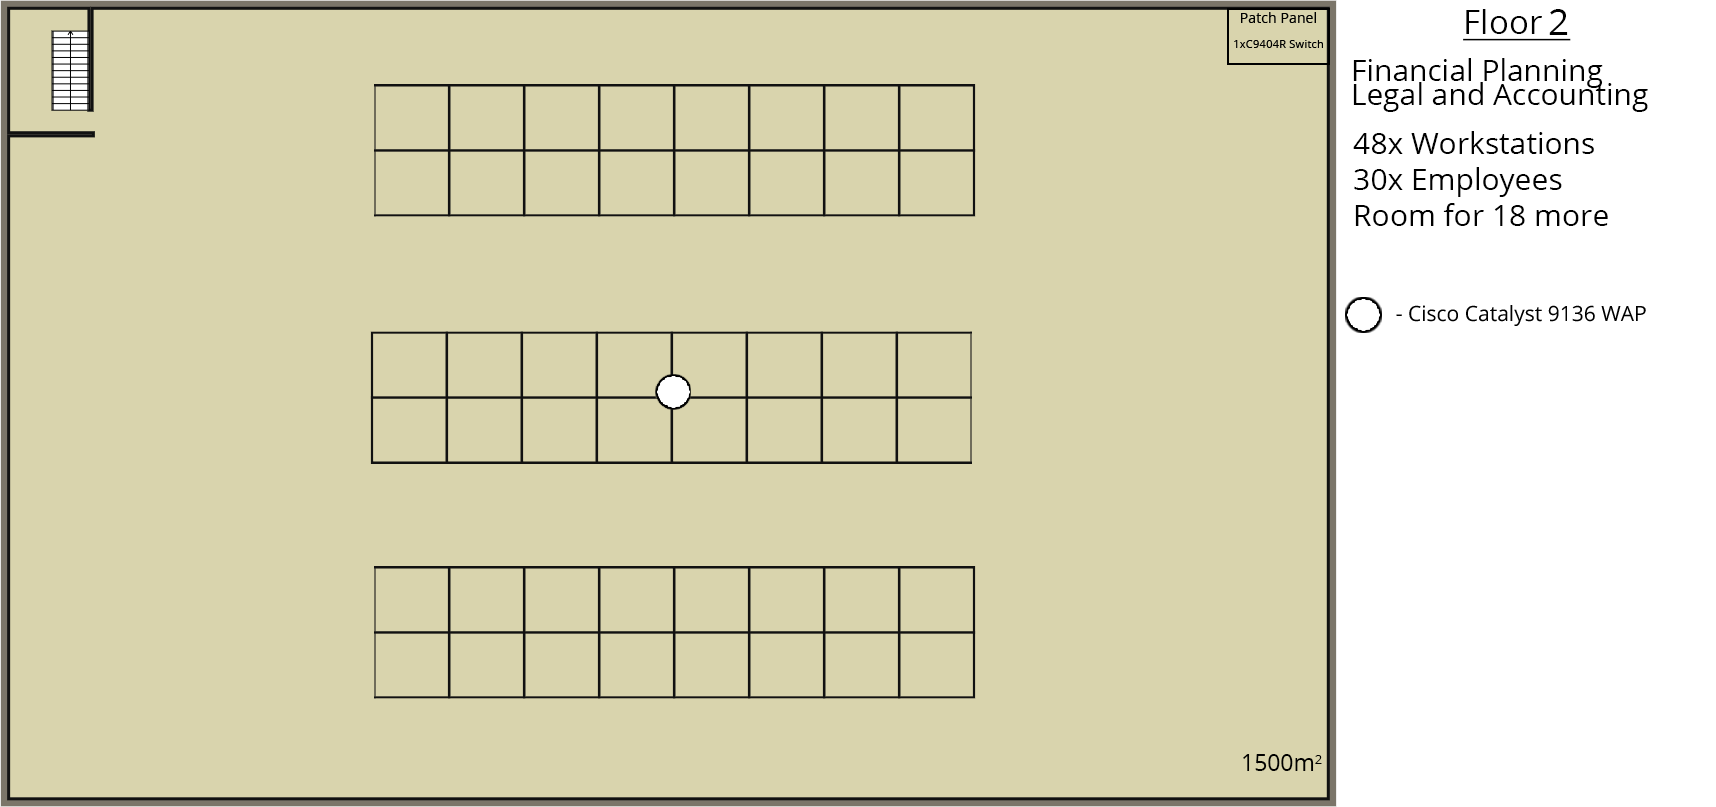
\includegraphics[width=15cm]{Figures/2nd-floor.png}
    \caption{2nd floor plan}
    \label{fig:2nd_floor}
\end{figure}
\subsection{3rd Floor}
\begin{figure}[H]
    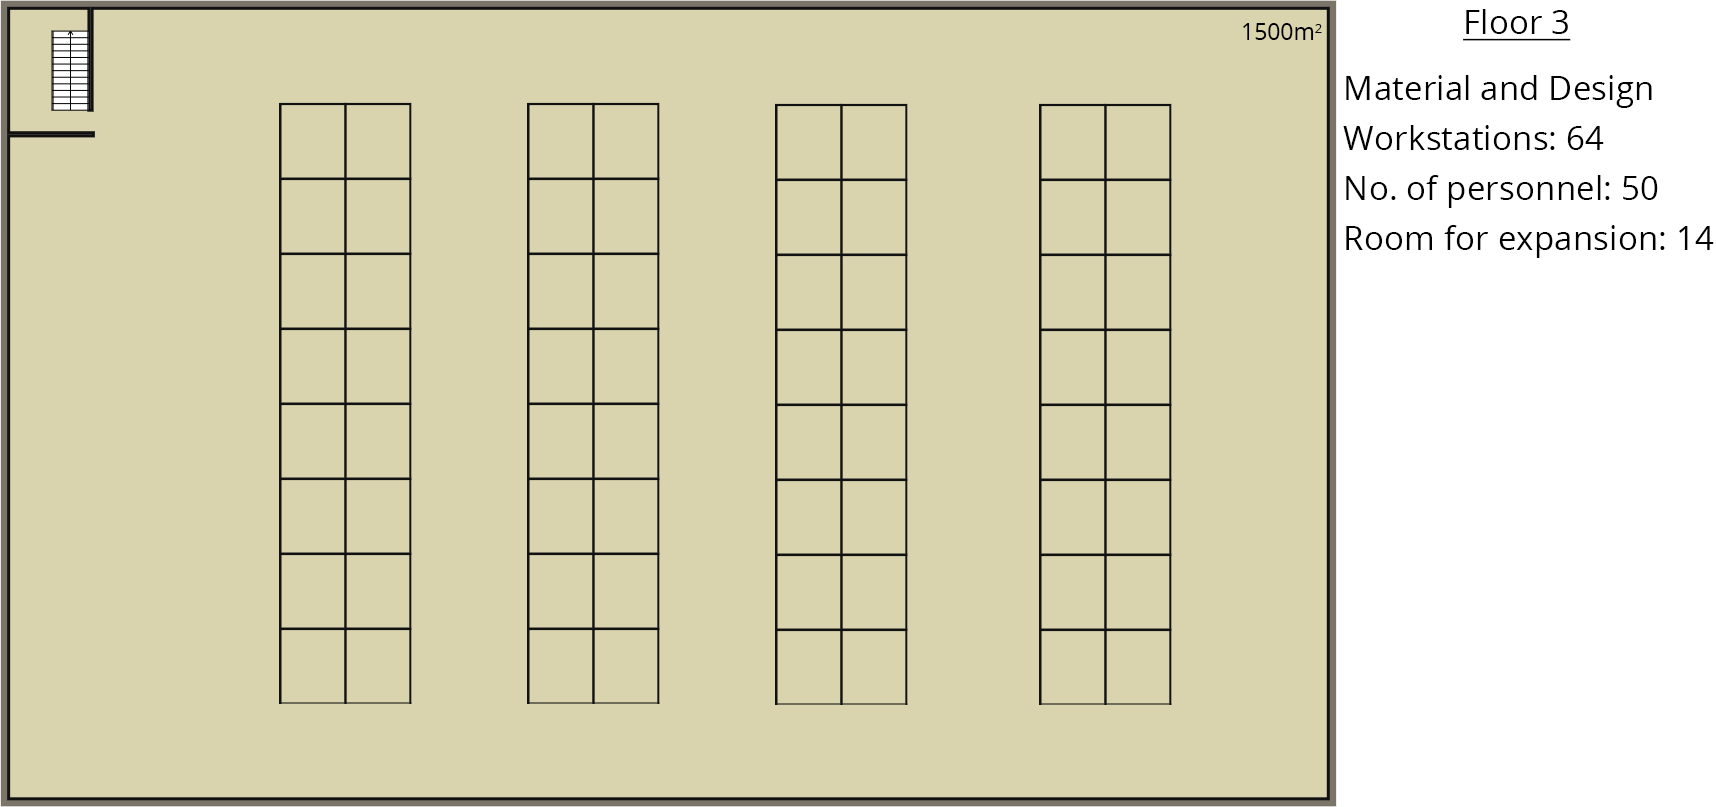
\includegraphics[width=15cm]{Figures/3rd-Floor.png}
    \caption{3rd floor plan}
    \label{fig:3rd_floor}
\end{figure}
\subsection{4th Floor}
\begin{figure}[H]
    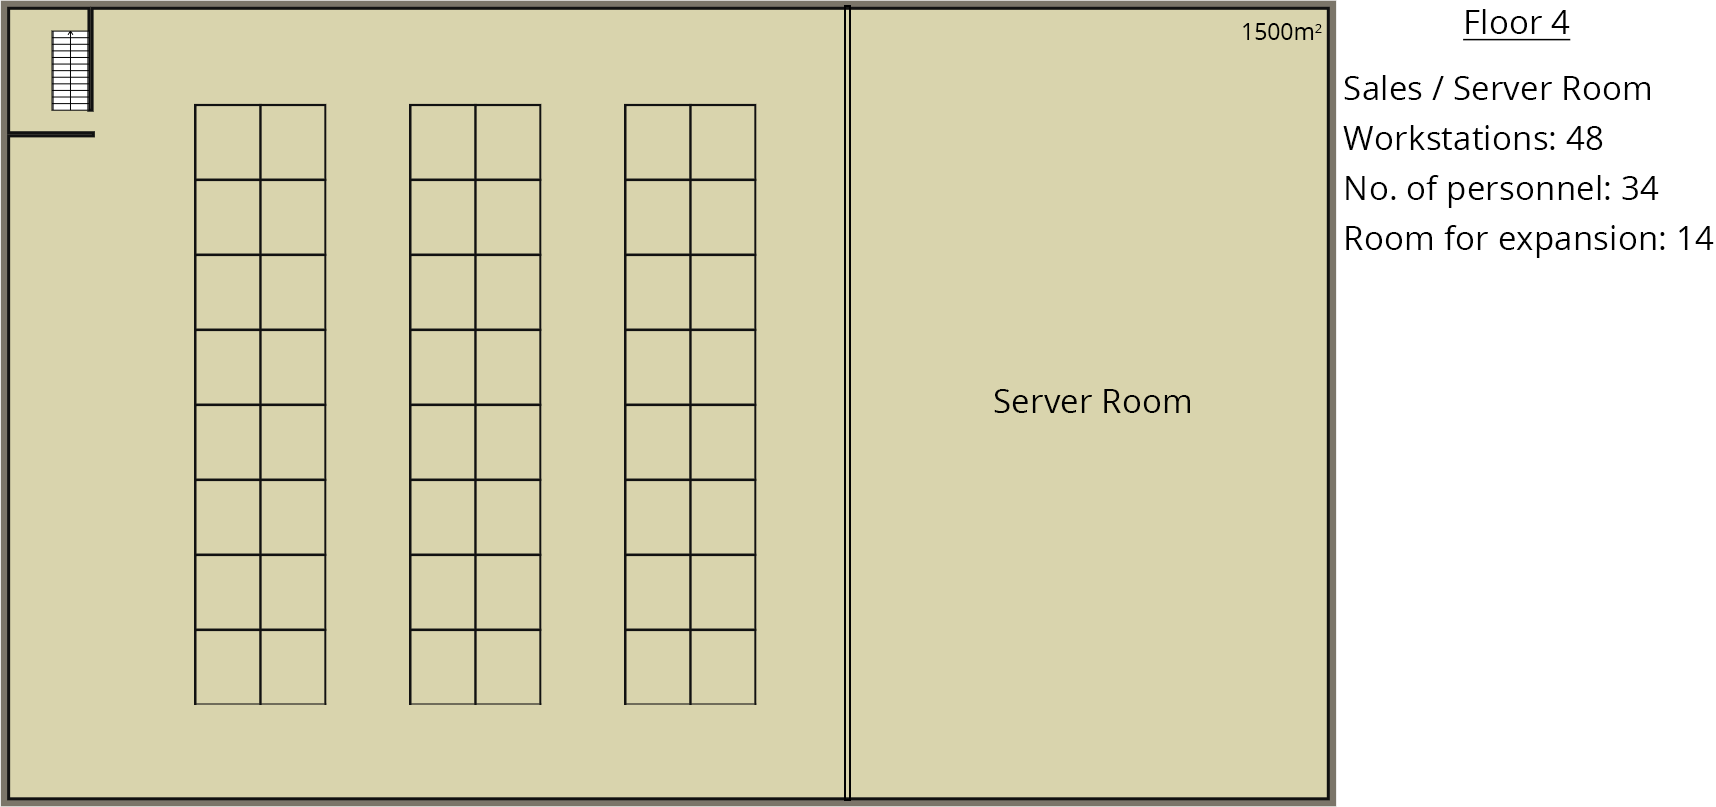
\includegraphics[width=15cm]{Figures/4th-Floor.png}
    \caption{4th floor plan}
    \label{fig:4th_floor}
\end{figure}
Explain why server room here
\subsection{5th Floor}
\begin{figure}[H]
    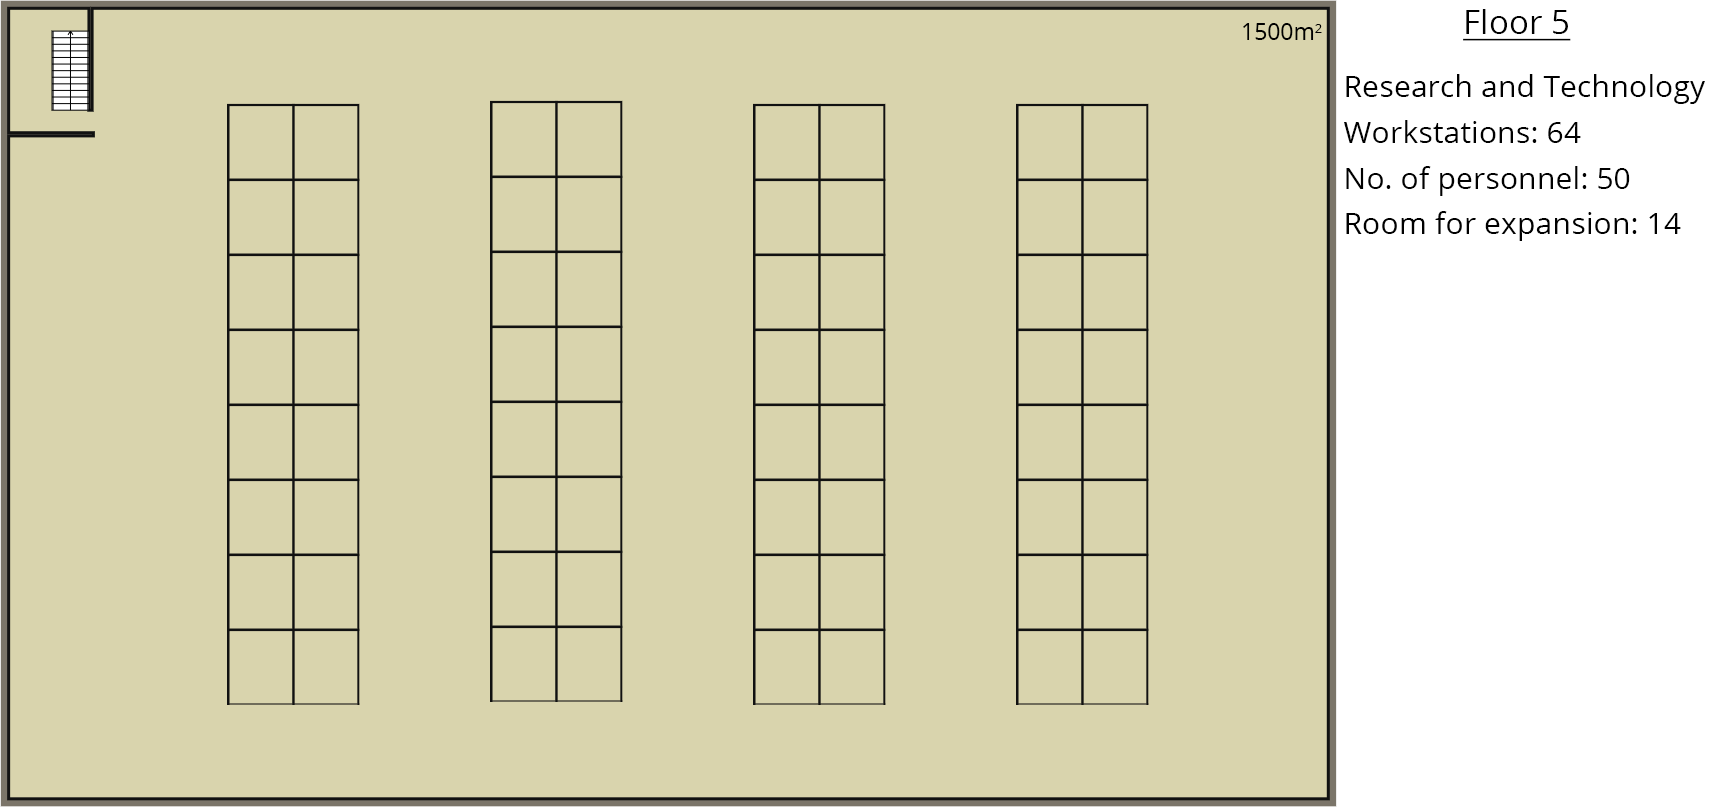
\includegraphics[width=15cm]{Figures/5th-Floor.png}
    \caption{5th floor plan}
    \label{fig:5th_floor}
\end{figure}
\subsection{6th Floor}
\begin{figure}[H]
    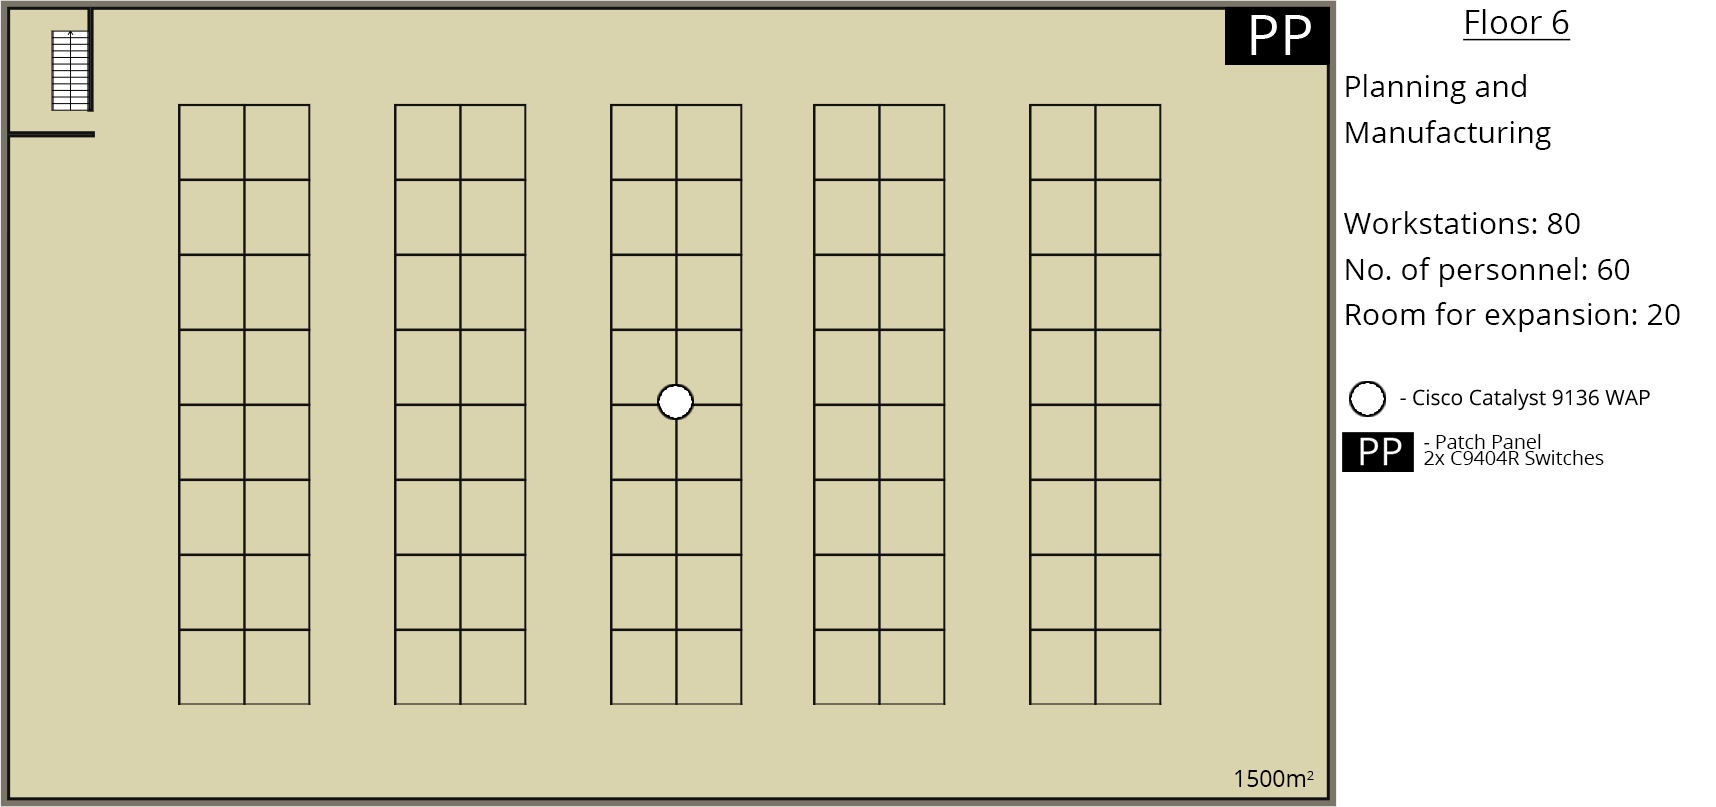
\includegraphics[width=15cm]{Figures/6th-Floor.png}
    \caption{6th floor plan}
    \label{fig:6th_floor}
\end{figure}
\subsection{7th Floor}
\begin{figure}[H]
    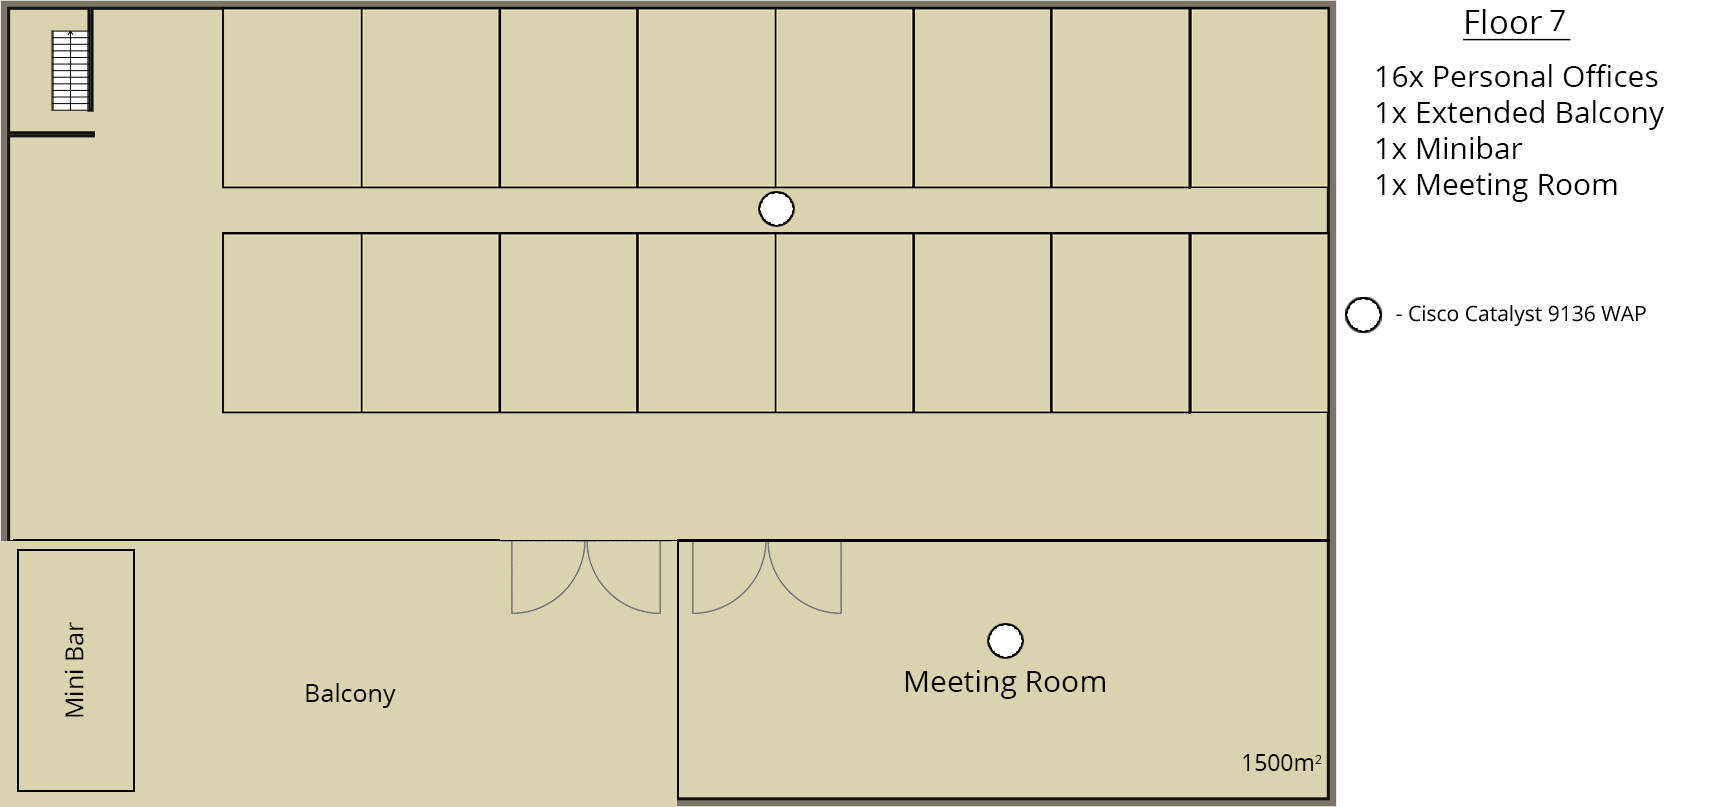
\includegraphics[width=15cm]{Figures/7th-floor.png}
    \caption{7th floor plan}
    \label{fig:7th_floor}
\end{figure}
\subsection{Server Room}
% \begin{figure}
%     \centering
%     \includegraphics[width=15cm]{Figures/}
%     \caption{Server racks diagram}
%     \label{fig:}
% \end{figure}
\chapter{Logical Network Design}

\begin{figure}[ht]
    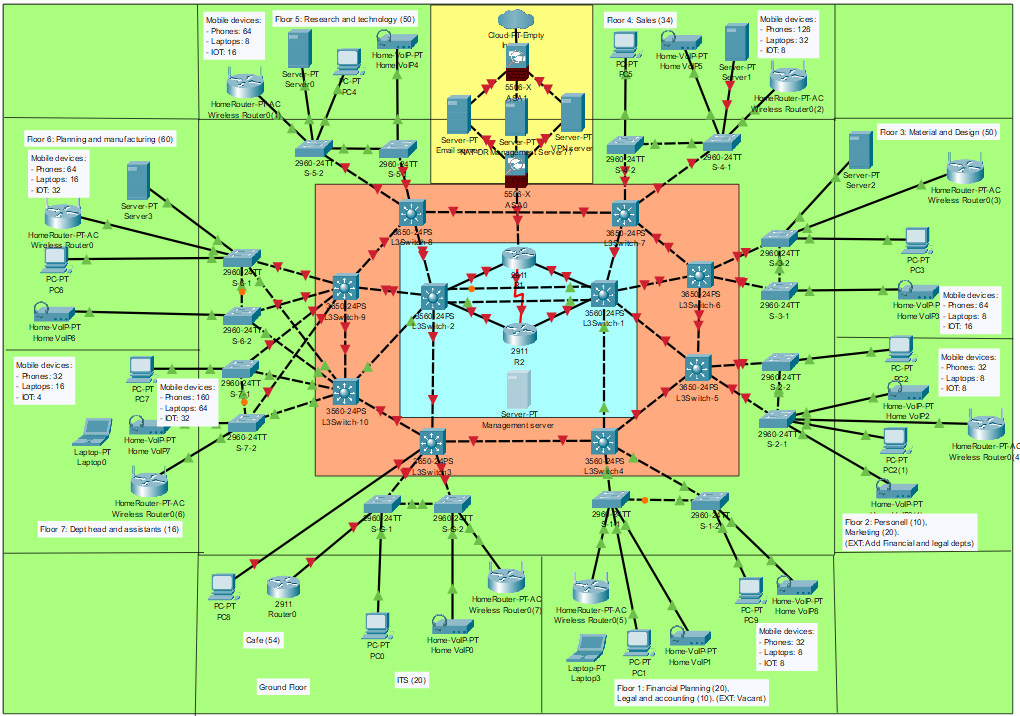
\includegraphics[width=15cm]{Figures/Network_Diagram.png}
    \caption{A Network Design produced in PacketTracer.}
    \label{fig:Network_Diagram}
\end{figure}

\section{Justifications}
\chapter{Addressing Scheme}

\begin{huge}
    NAT/PAT enabled
\end{huge}

Ground Floor:\\
IT Dept: 10.0.1.0\\
Cafe:    10.0.2.0\\
Wireless: 10.0.3.0\\
Phones: 10.0.4.0\\

Floor 1:\\
Financial Planning: 10.1.1.0\\
Legal \& accounting: 10.1.2.0\\
Wireless: 10.1.3.0\\
Phones: 10.1.4.0\\

Floor 2:\\
Personell: 10.2.1.0\\
Marketing: 10.2.2.0\\
Wireless: 10.2.3.0\\
Phones: 10.2.4.0\\

Floor 3:\\
Material and Design: 10.3.1.0\\
Wireless: 10.3.2.0\\
Phones: 10.3.3.0\\

Floor 4:\\
Sales: 10.4.1.0\\
Wireless: 10.4.2.0\\
Phones: 10.4.3.0\\

Floor 5:\\
Research and Tech: 10.5.1.0\\
Wireless: 10.5.2.0\\
Phones: 10.5.3.0\\

Floor 6:\\
Planning and Manufacturing: 10.6.1.0\\
Wireless: 10.6.2.0\\
Phones: 10.6.3.0\\

Floor 7:\\
Dept Heads \& Assistants: 10.7.1.0\\
Wireless: 10.7.2.0\\
Phones: 10.7.3.0\\

Underground:\\
Wireless\\

\chapter{Network Policies}

\section{Work issued hardware}
\begin{itemize}
    \item Cannot be left unnatened
    \item Should donly be used for work purposes
    \item Every quater all work issued hardware should be handed back for security inspections and log analysis
\end{itemize}

\section{backups}
\begin{itemize}
    \item all server infrastructure shoul be backed up on a regular basis
    \item 
\end{itemize}

\section{New Infrastructure}
\begin{itemize}
    \item Any new server infrastructure should be installed inside the network DMZ
\end{itemize}

\section{Personal Devices}
\begin{itemize}
    \item personal devices should be ensured to have a sufficient level of anti-virus
\end{itemize}


\chapter{Security}

\section{Overview}
As Yotsuba Group is a large manufacturing company leading the market in Asia, their assets and infrastructure are a prime target for cyber-attacks. The manufacturing industry is reported as the 2nd most targeted industry by cyber attackers, primarily due to COVID-19 \parencite{top7-BitLyft} so ensuring that Yotsuba Group can cope with these threats is crucial.
\section{Identifying Network Security Threats}
\subsection{MAC Spoofing}
 MAC spoofing is a common layer 2 attack that forges a suspicious MAC address as a legitimate one. Due to this, a suspicious device can then bypass security controls to access the network \parencite{mac-spoofing}.
ARP Cache Poisoning: Similarly, common layer 3 attacks include ARP cache poisoning. This attack takes advantage of the insecure nature of the ARP protocol and potentially leads to man-in-the-middle attacks. Since the ARP protocol doesn't verify identities, it can be easy for an attacker to trick a legitimate host into thinking its legitimate itself. Therefore, if an ARP poisoning attack is successful, the attacker can view all traffic sent between two hosts \parencite{arp-posioning} check.
\subsection{Static VLAN Security}
Insecurities of static VLAN switches could lead to an attacker being able to connect to a VLAN by simply connecting their device to a switch. If successful, an attacker would be able to communicate to other devices in the VLAN as well as accessing potentially sensitive data.

\section{Mitigation}
\subsection{Device Security}
At the very least, YG should implement a strong password policy and multi-factor authentication. This is basic level security but prevents even the simplest of attacks. Unnecessary services and applications should also be disabled on devices that do not need them to protect the network from vulnerabilities in certain applications. For example, employees in the manufacturing department will not need access to finance applications, so segregating them makes the network more robust.
\subsection{Port Security}
Sticky MAC addressing. A switch will learn a MAC address that corresponds to a specific port. In sticky learning, this is remembered even after a reboot. Introducing sticky MAC address learning means a device that is not recognised will not be allowed into the network.
\subsection{ACLs and Firewalls}
Thorough Access Control Lists should be created to control network traffic. Having ACLs limits the lateral movement an attacker can make within a network by permitting or denying traffic from one host or group to another. Similarly, we have placed a firewall between the internet and internal network. The firewall protects the network by filtering incoming packets and decides whether to drop the packet based off a predefined set of rules \parencite{cisco-firewall}.
\subsection{Static ARP Tables}
Manually configuring ARP tables means that MAC addresses can be statically mapped to their corresponding IP address. Doing this is a highly effective method to prevent ARP poisoning attacks, although requires a lot of time to complete \parencite{arp-posioning}. 

\section{Previous Security Threats}
The Yotsuba Group reported a number of security incidents in the last 6 months. These have been assumed below.
\subsection{IP Theft}
The company had some intellectual property stolen from a physical attack on the servers within the company premises, the attackers were not found or apprehended as the security was not to standard. This attack was made possible by a lack of physical security measures on there network infrastructure.
\subsection{Internal Breach}
30\% of attacks come from employee’s within the companies, some data was accessed by departments who has access to other parts of the organisation that they should not have had. A lack of access control was the cause of this attack.
\subsection{Identity Theft}
An external attack left the customer database held by the company open and accessible to the attackers, this in turn was used to ciphon their data and initiate fraud through loan applications under customer names.
\chapter{Monitoring and Maintenance}

\section{Software}

\section{Justifications}

\chapter{Disaster Plan}
\section{Outline and Scope}
This disaster management and contingency plan aims to identify risks and provide methods of mitigation. Certain network issues can be treated with automation via the setup of executables using the Intermapper network management software. If manual intervention is required, the plan employs a systematic approach, which allows problems to be treated in a sufficient timeframe, but with enough knowledge so that it can be understood and corrected properly. We have been proactive with our network design, employing the Cisco 3-layer hierarchical model to prevent issues and help with troubleshooting. Our design makes it easier to isolate a section of the network where an issue may be found, makes scaling easier and ensures we have redundancy within the network.
\section{Risks and Mitigation}
\begin{table}[H]
    \centering
    \begin{tabular}{|p{0.35\linewidth}|p{0.35\linewidth}|p{0.35\linewidth}|}
    \hline
    Risk                                                 & Potential Consequences                                                                                       & Mitigation                                                                                                                                                                                                                         \\ \hline
    Natural Disaster i.e., flooding, earthquake, tsunami & Destruction of the building or critical IT infrastructure. Loss of critical personal and manufacturing data. & Seek cloud-based computing solutions for storage of critical data in geographical locations where natural disasters are less frequent.                                                                                             \\ \hline
    Fire                                                 & Destruction or damage to critical IT infrastructure. Damage to company reputation                            & Conduct regular fire assessments, ensuring sockets are PAT tested and fire extinguishers are readily available.                                                                                                                    \\ \hline
    Power Cut                                            & Disrupt operations and potential loss of data.                                                               & Utilise the space in the underground car park for a temporary backup power supply. Ensure this power supply can handle normal business operations.                                                                                 \\ \hline
    Network Issues                                       & Loss of communications and disruption of operations.                                                         & Ensure adequate levels of redundancy are implemented into the network. Isolate network where the issue is and ensure there is enough backup equipment available to create a simple network should critical operations be required. \\ \hline
    Theft                                                & Loss of infrastructure or crucial data. Damage to reputation.                                                & Ensure IT team performs regular checks on IT devices along with trackers and encrypted hardware.                                                                                                                                   \\ \hline
    Software Issues                                      & Disruption of operations. Loss of access to data.                                                            & Perform backups regularly before updating software. If the latest versions of software cause issues, the IT team should roll back to the previous version if there is no significant vulnerability risk.                           \\ \hline
    Hardware Issues                                      & Disruption of operations. Loss of access to data.                                                            & Planned resolution methods for each network device, whether it is router, switch or computer. Isolate network where hardware issue is if needed and perform regular backups to prevent loss of data.                               \\ \hline
    Employee Lost Device                                 & Possible loss of data and/or exposure of sensitive company data.                                             & Ensure password policies are enforced on employee devices, with multi-factor authentication and encrypted hard drives.                                                                                                             \\ \hline
    \end{tabular}
    \caption{Risks and mitigations}
    \label{tab:risks_mitigations}
\end{table}

\section{Risk Assessment Matrix}

The Risk Assessment Matrix provides visual indication of how likely a risk is to occur, as well as its impact on Yotsuba Group in such an event. Mitigation methods described in Table \ref{tab:risks_mitigations} will help overcome and reduce the consequences of these risks.

\begin{figure}[H]
    \centering
    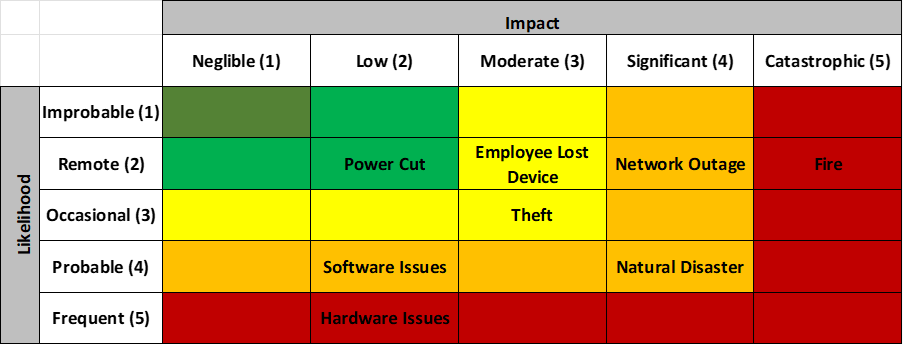
\includegraphics[width=15cm]{Figures/risk_assessment_matrix.png}
    \caption{Risk assessment matrix for Yotsuba Group}
    \label{fig: table}
\end{figure}
\chapter{Additional Problems}

\section{Renting One Floor Out}

The second floor will combine four different departments to allow for space in the first floor. The new layout can be seen in figure \ref{fig:2nd_floor_varient}.
\begin{figure}[!h]
    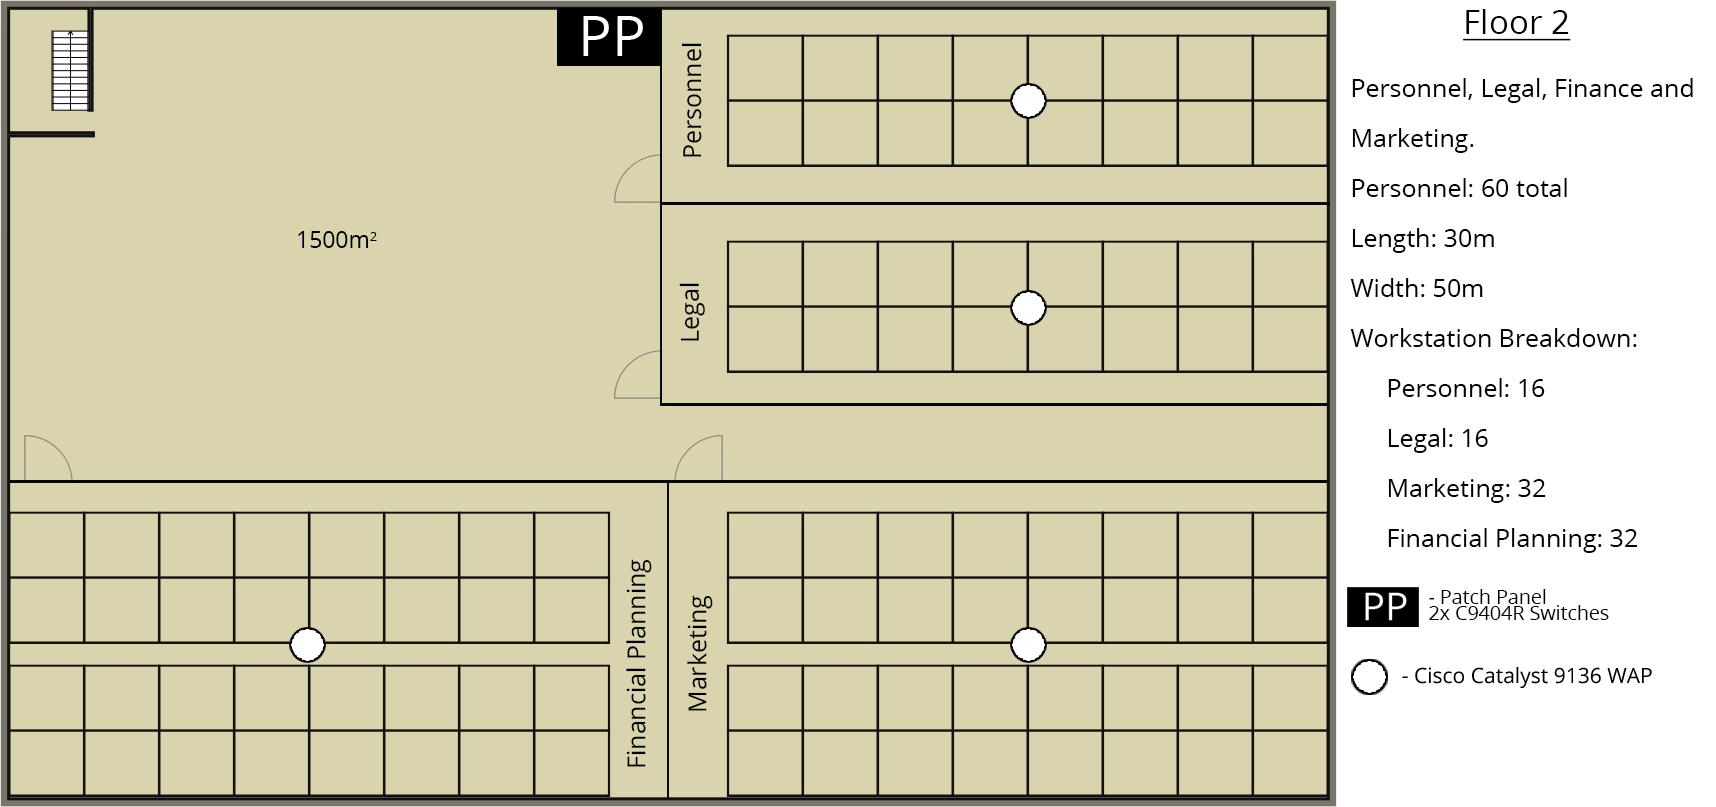
\includegraphics[width=15cm]{Figures/2nd-Floor-Varient.png}
    \caption{2nd floor plan combining 4 different departments}
    \label{fig:2nd_floor_varient}
\end{figure}

\begin{figure}[h]
    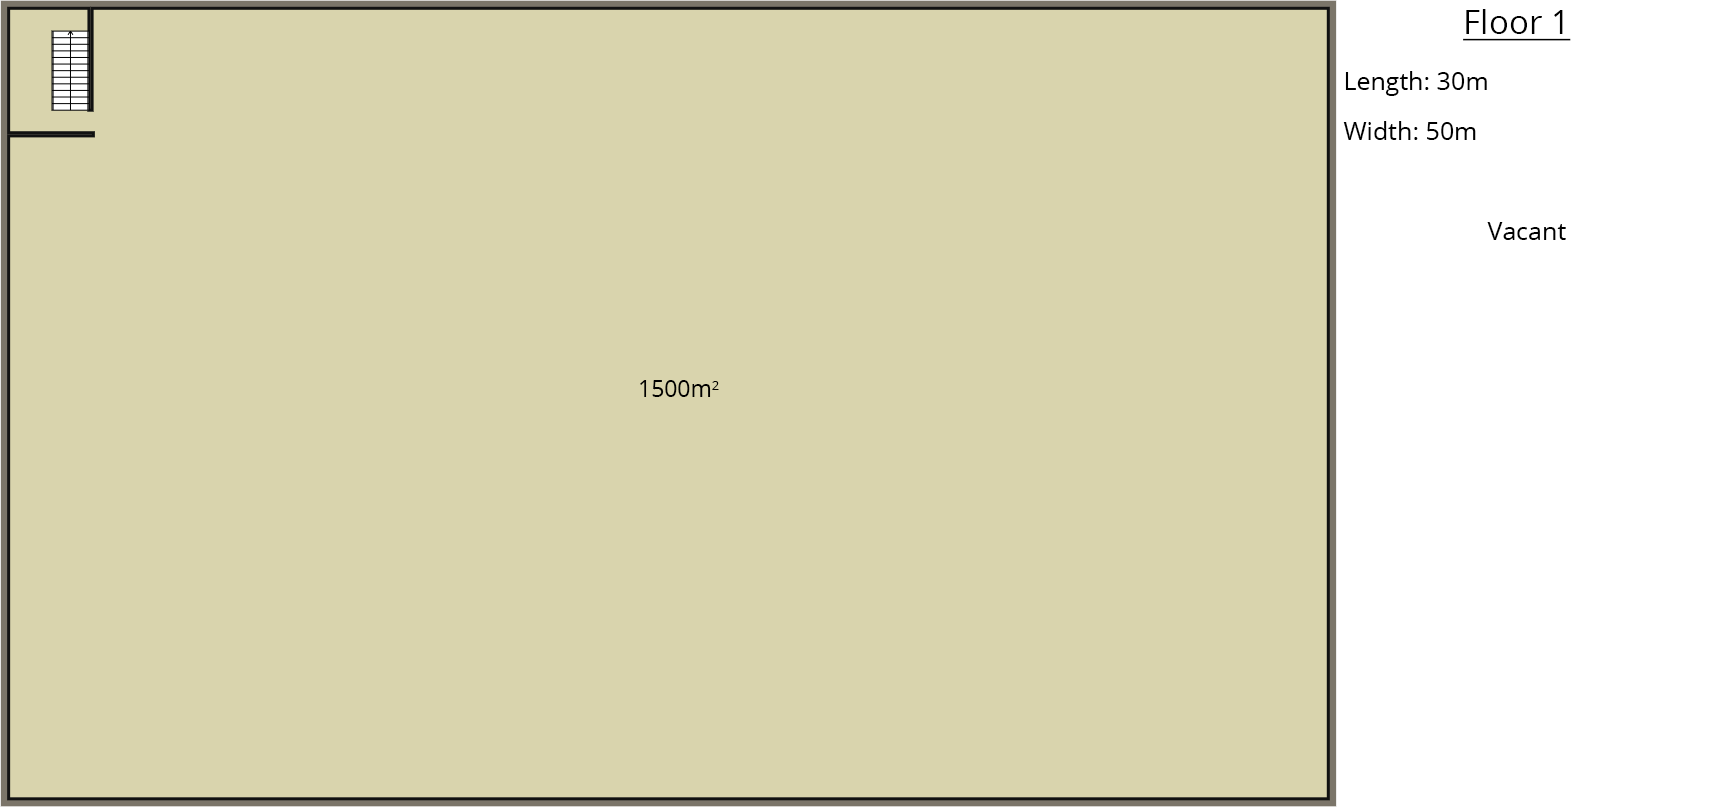
\includegraphics[width=15cm]{Figures/1st-Floor-varient.png}
    \caption{1st floor vacant plan}
    \label{fig:1st_floor_empty}
\end{figure}

The design and addressing specifications sections 4 and 5 are able to be reconfigured to place the occupants of floor 1 (currently financial planning and legal and accounting) and place them physically and logically on floor 2. This would include them being on the floor 2 subnet and no longer connected to floor 1. This vacant floor is then available for renting and is segregated on its own network.

\section{Splitting Between Two Buildings}
The servers that are able to give access to VPN and email are located within the DMZ, these will be accessible from the old HQ building network if Yotsuba decide to use it. The addressing scheme also allows the possiblity of adding many more devices to the internal network structure, so if they were to run the cabling between the buildings it could be incorporated directly. 
Running Single mode fiber between buildings.

\clearpage

% References
\addcontentsline{toc}{chapter}{References}
\printbibliography
\end{document}